\documentclass[a4paper, 12pt]{article}%тип документа

\usepackage{placeins}
%отступы
\usepackage[left=2cm,right=2cm,top=2cm,bottom=3cm,bindingoffset=0cm]{geometry}

%Русский язык
\usepackage[T2A]{fontenc} %кодировка
\usepackage[utf8]{inputenc} %кодировка исходного кода
\usepackage[english,russian]{babel} %локализация и переносы

%Вставка картинок
\usepackage{wrapfig}
\usepackage{graphicx}
\graphicspath{{pictures/}}
\DeclareGraphicsExtensions{.pdf,.png,.jpg}

%Графики
\usepackage{multirow}
\usepackage{pgfplots}
\pgfplotsset{compat=1.9}

%Математика
\usepackage{amsmath, amsfonts, amssymb, amsthm, mathtools}

%Заголовок
\author{Валеев Рауф Раушанович \\
группа 825}
\title{\textbf{Работа 2.2.3 \\ 
Измерение теплопроводности воздуха при атмосферном давлении}}
\begin{document}
\maketitle
\newpage
\section*{Теоретическая справка}
\textit{Теплопроводность} — это процесс передачи тепловой энергии от нагретых частей системы к холодным за счёт хаотического движения частиц среды (молекул, атомов и т.п.). В газах теплопроводность осуществляется за счёт  непосредственной передачи кинетической энергии от быстрых молекул к медленным при их столкновениях. Перенос тепла описывается законом Фурье, утверждающим, что плотность потока энергии $\overline{q} = -k \nabla T$, где $k \left[ \dfrac{\text{Вт}}{\text{м} \cdot \text{К}} \right]$ - \textit{коэффициент теплопроводности}.

Молекулярно-кинетическая теория дает следующую оценку для коэффициента теплопроводности газов: 
\[k \sim \lambda \overline{\nu} \cdot n c_V\]
С помощью некоторых преобразований мы получаем, что 
\[ Q = \dfrac{2 \pi L}{\ln \dfrac{r_0}{r_1}} k  \cdot \Delta T \]
\section*{Экспериментальная установка}
\begin{wrapfigure}{r}{0.4\textwidth}
  \begin{center}
    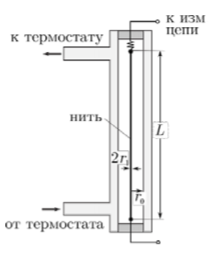
\includegraphics[width = 0.3\textwidth]{7.png}
  \end{center}
  \textbf{\caption{Схема установки}}
\end{wrapfigure}
Схема установки приведена на рис. 1. На оси полой цилиндрической трубки с внутренним диаметром $2r_0 \sim 1$ см размещена металлическая нить диаметром $2r_1 \sim 0,05$ мм и длиной $L \sim 40$ см (материал нити и точные геометрические размеры указаны в техническом описании установки). Полость трубки заполнена воздухом (полость через небольшое отверстие сообщается с атмосферой). Стенки трубки помещены в кожух, через которых пропускается вода из термостата, так что их температура $t_0$ поддерживается постоянной. Для предотвращения конвекции трубка расположена вертикально.

Металлическая нить служит как источником тепла, так и датчиком температуры (термометром сопротивления). По пропускаемому через нить постоянному току $I$ и напряжению $U$ на ней вычисляется мощность нагрева по закону Джоуля–Ленца: $Q = UI$, и сопротивление нити по закону Ома: $R = \dfrac{U}{I}$.

Сопротивление нити является однозначной функцией её температуры $R (t)$.
Эта зависимость может быть измерена с помощью термостата по экстраполяции мощности нагрева к нулю $Q \rightarrow 0$, когда температура нити и стенок совпадают $t_1 \approx t_0$. Альтернативно, если материал нити известен, зависимость его удельного сопротивления от температуры может найдена по справочным данным.
\newpage
На рис. 2 представлена схема электрической установки:
\begin{wrapfigure}{r}{0.6\textwidth}
  \begin{center}
    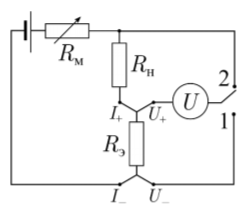
\includegraphics[width = 0.5\textwidth]{8.png}
  \end{center}
  \textbf{\caption{Электрическая схема измерения сопротивления нити и мощности нагрева}}
\end{wrapfigure}
Схема рис. 2 предусматривает использование одного вольтметра и эталонного сопротивления $R_{\text{э}} \sim 10$ Ом (точное значение $R_{\text{э}}$ и его класс точности указаны в техническом описании установки), включённого последовательно с нитью. В положении переключателя 2 вольтметр измеряет напряжение на нити, а в положении 1 — напряжение на $R_{\text{э}}$, пропорциональное току через нить. Для исключения влияния контактов и подводящих проводов эталонное сопротивление $R_{\text{э}}$ также необходимо подключать в цепь по четырёхпроводной схеме. Ток в цепи в обеих схемах регулируется с помощью реостата или магазина сопротивлений $R_{\text{м}}$, включённого последовательно с источником напряжения.
\section*{Методика измерений} 
Принципиально неустранимая систематическая ошибка измерения температуры с помощью термометра сопротивления возникает из-за необходимости пропускать через резистор (нить) измерительный ток. Чем этот ток выше, тем с большей точностью будет измерен как он сам, так и напряжение. Однако при этом квадратично возрастает выделяющаяся на  резисторе мощность $Q = UI = I^2R$. Следовательно, температура резистора становится выше, чем у объекта, температуру которого надо измерить. Измерения же при малых токах не дают достаточной точности (в частности, из-за существенного вклада термоэлектрических явлений в проводниках и контактах). Эта проблема решается построением нагрузочной кривой - зависимости измеряемого сопротивления $R$ от выделяющейся в нём мощности $R(Q)$, с последующей экстраполяцией к нулевой мощности $Q \to 0$ для определения сопротивления $R_0 = R(0)$, при котором его температура равна температуре измеряемого объекта. Кроме того, в данной работе измерение нагрузочных кривых позволяет в ходе эксперимента получить температурную зависимость сопротивления нити, так как при $Q \to 0$ температура нити равна температуре термостата ($T \approx T_0$). В исследуемом интервале температур (20-70 $^0C$) зависимость сопротивления от температуры можно с хорошей точностью аппроксимировать линейной функцией:
\[R(t) = R_{273} \cdot (1 + \alpha t)\]
где $\alpha = \dfrac{1}{R_{273}} \dfrac{dR}{dT}$ - температурный коэффициент сопротивления материала.
\section*{Ход работы}
\begin{enumerate}
\item При комнатной температуре термостата измеряем зависимость сопротивления нити $R =\dfrac{U}{I}$ от подаваемой на неё мощности $Q = UI$ - нагрузочную кривую $R(Q)$.

Измерения проводим для 7-9 различных значений силы тока через нить от 0 до $I_{max}$.
\begin{table}[h]
\begin{center}
\begin{tabular}{|c|c|c|c|}
\hline
\multicolumn{4}{|c|}{$T = 25 ^0 C$} \\ \hline
$Q, 10^{-6}$ Дж & $\sigma_Q, 10^{-6}$ Дж & $R$, Ом & $\sigma_R$, Ом \\ \hline
0,0143 & 0,0001 & 11 & 0,01 \\ \hline
0,0174 & 0,0001 & 11,03 & 0,01 \\ \hline
0,0211 & 0,0001 & 11,05 & 0,01 \\ \hline
0,0268 & 0,0001 & 11,06 & 0,01 \\ \hline
0,0348 & 0,0001 & 11,11 & 0,01 \\ \hline
0,0471 & 0,0001 & 11,14 & 0,01 \\ \hline
0,0670 & 0,0001 & 11,16 & 0,01 \\ \hline
0,1033 & 0,0001 & 11,19 & 0,01 \\ \hline
0,1806 & 0,0001 & 11,20 & 0,01 \\ \hline
\end{tabular}
\end{center}
\caption{Данные для комнатной температуры}
\end{table} 
\item Проводим измерения нагрузочных кривых согласно п. 1 для 5–7 температур термостата в диапазоне от комнатной до 70 $^0 C$.
\begin{table}[h]
\begin{center}
\begin{tabular}{|c|c|c|c|}
\hline
\multicolumn{4}{|c|}{$T = 35 ^0 C$} \\ \hline
$Q, 10^{-6}$ Дж & $\sigma_Q, 10^{-6}$ Дж & $R$, Ом & $\sigma_R$, Ом \\ \hline
0,0149 & 0,0001 & 11,09 & 0,01 \\ \hline
0,0180 & 0,0001 & 11,14 & 0,01 \\ \hline
0,0221 & 0,0001 & 11,14 & 0,01 \\ \hline
0,0280 & 0,0001 & 11,20 & 0,01 \\ \hline
0,0363 & 0,0001 & 11,193 & 0,01 \\ \hline
0,0491 & 0,0001 & 11,22 & 0,01 \\ \hline
0,0703 & 0,0001 & 11,27 & 0,01 \\ \hline
0,1086 & 0,0001 & 11,32 & 0,01 \\ \hline
0,1898 & 0,0001 & 11,34 & 0,01 \\ \hline
\end{tabular}
\end{center}
\caption{Данные для $T = 35 ^0 C$}
\end{table}
\FloatBarrier
\begin{table}[h]
\begin{center}
\begin{tabular}{|c|c|c|c|}
\hline
\multicolumn{4}{|c|}{$T = 45 ^0 C$} \\ \hline
$Q, 10^{-6}$ Дж & $\sigma_Q, 10^{-6}$ Дж & $R$, Ом & $\sigma_R$, Ом \\ \hline
0,0153 & 0,0001 & 11,51 & 0,01 \\ \hline
0,0185 & 0,0001 & 11,52 & 0,01 \\ \hline
0,0229 & 0,0001 & 11,57 & 0,01 \\ \hline
0,0288 & 0,0001 & 11,58 & 0,01 \\ \hline
0,0379 & 0,0001 & 11,67 & 0,01 \\ \hline
0,0507 & 0,0001 & 11,68 & 0,01 \\ \hline
0,0724 & 0,0001 & 11,69 & 0,01 \\ \hline
0,1121 & 0,0001 & 11,70 & 0,01 \\ \hline
0,1960 & 0,0001 & 11,71 & 0,01 \\ \hline
\end{tabular}
\end{center}
\caption{Данные для $T = 45 ^0 C$}
\end{table}
\FloatBarrier
\FloatBarrier
\begin{table}[h]
\begin{center}
\begin{tabular}{|c|c|c|c|}
\hline
\multicolumn{4}{|c|}{$T = 55 ^0 C$} \\ \hline
$Q, 10^{-6}$ Дж & $\sigma_Q, 10^{-6}$ Дж & $R$, Ом & $\sigma_R$, Ом \\ \hline
0,0159 & 0,0001 & 11,95 & 0,01 \\ \hline
0,0191 & 0,0001 & 11,95 & 0,01 \\ \hline
0,0236 & 0,0001 & 11,96 & 0,01 \\ \hline
0,0301 & 0,0001 & 11,98 & 0,01 \\ \hline
0,0386 & 0,0001 & 11,99 & 0,01 \\ \hline
0,0524 & 0,0001 & 12,00 & 0,01 \\ \hline
0,0749 & 0,0001 & 12,00 & 0,01 \\ \hline
0,1157 & 0,0001 & 12,05 & 0,01 \\ \hline
0,2019 & 0,0001 & 12,10 & 0,01 \\ \hline
\end{tabular}
\end{center}
\caption{Данные для $T = 55 ^0 C$}
\end{table}
\FloatBarrier
\FloatBarrier
\begin{table}[h]
\begin{center}
\begin{tabular}{|c|c|c|c|}
\hline
\multicolumn{4}{|c|}{$T = 65 ^0 C$} \\ \hline
$Q, 10^{-6}$ Дж & $\sigma_Q, 10^{-6}$ Дж & $R$, Ом & $\sigma_R$, Ом \\ \hline
0,0165 & 0,0001 & 12,30 & 0,01 \\ \hline
0,0198 & 0,0001 & 12,35 & 0,01 \\ \hline
0,0243 & 0,0001 & 12,37 & 0,01 \\ \hline
0,0307 & 0,0001 & 12,39 & 0,01 \\ \hline
0,0400 & 0,0001 & 12,39 & 0,01 \\ \hline
0,0543 & 0,0001 & 12,42 & 0,01 \\ \hline
0,0776 & 0,0001 & 12,43 & 0,01 \\ \hline
0,1198 & 0,0001 & 12,47 & 0,01 \\ \hline
0,2089 & 0,0001 & 12,50 & 0,01 \\ \hline
\end{tabular}
\end{center}
\caption{Данные для $T = 65 ^0 C$}
\end{table}
\FloatBarrier
\FloatBarrier
\begin{table}[h]
\begin{center}
\begin{tabular}{|c|c|c|c|}
\hline
\multicolumn{4}{|c|}{$T = 70 ^0 C$} \\ \hline
$Q, 10^{-6}$ Дж & $\sigma_Q, 10^{-6}$ Дж & $R$, Ом & $\sigma_R$, Ом \\ \hline
0,0206 & 0,0001 & 12,65 & 0,01 \\ \hline
0,0254 & 0,0001 & 12,76 & 0,01 \\ \hline
0,0321 & 0,0001 & 12,77 & 0,01 \\ \hline
0,0419 & 0,0001 & 12,77 & 0,01 \\ \hline
0,0569 & 0,0001 & 12,79 & 0,01 \\ \hline
0,0819 & 0,0001 & 12,80 & 0,01 \\ \hline
0,1280 & 0,0001 & 12,80 & 0,01 \\ \hline
0,2336 & 0,0001 & 13,11 & 0,01 \\ \hline
\end{tabular}
\end{center}
\caption{Данные для $T = 70 ^0 C$}
\end{table}
\FloatBarrier
\FloatBarrier
\begin{figure}[h]
\center{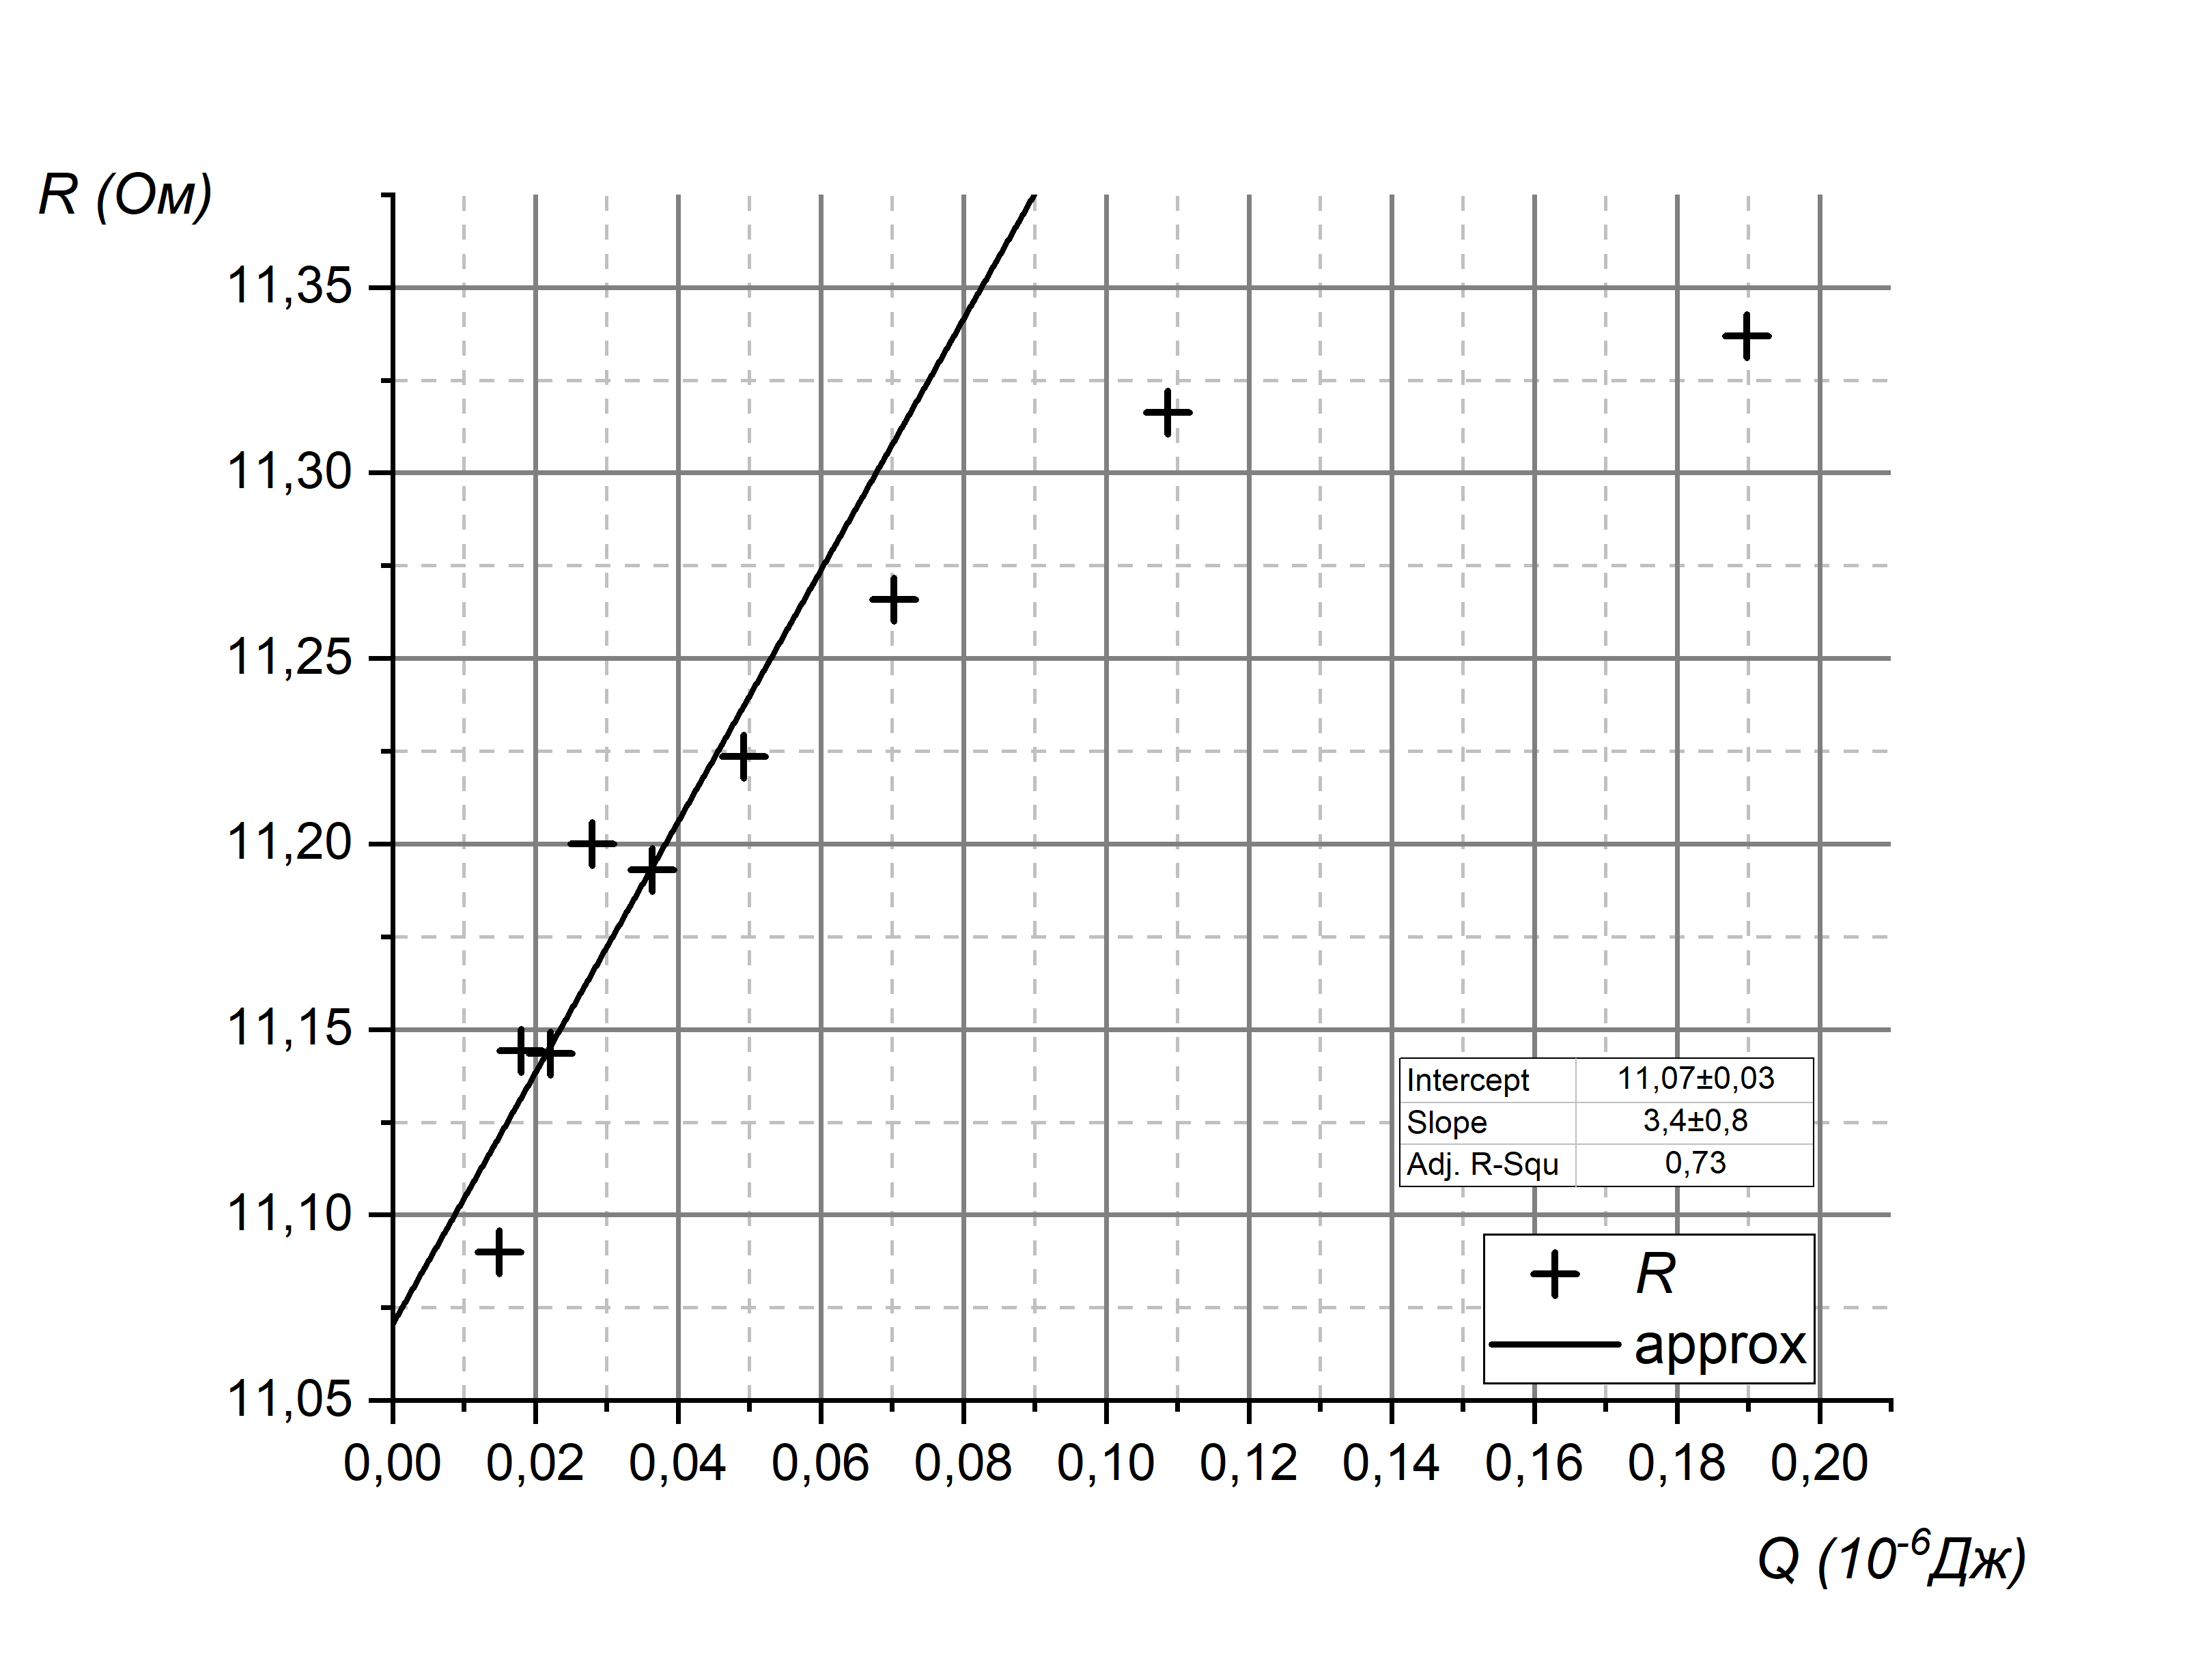
\includegraphics[width = 0.9\textwidth]{1.jpg}}
\caption{График для $T = 25 ^0 C$}
\end{figure}
\FloatBarrier
\FloatBarrier
\begin{figure}[h]
\center{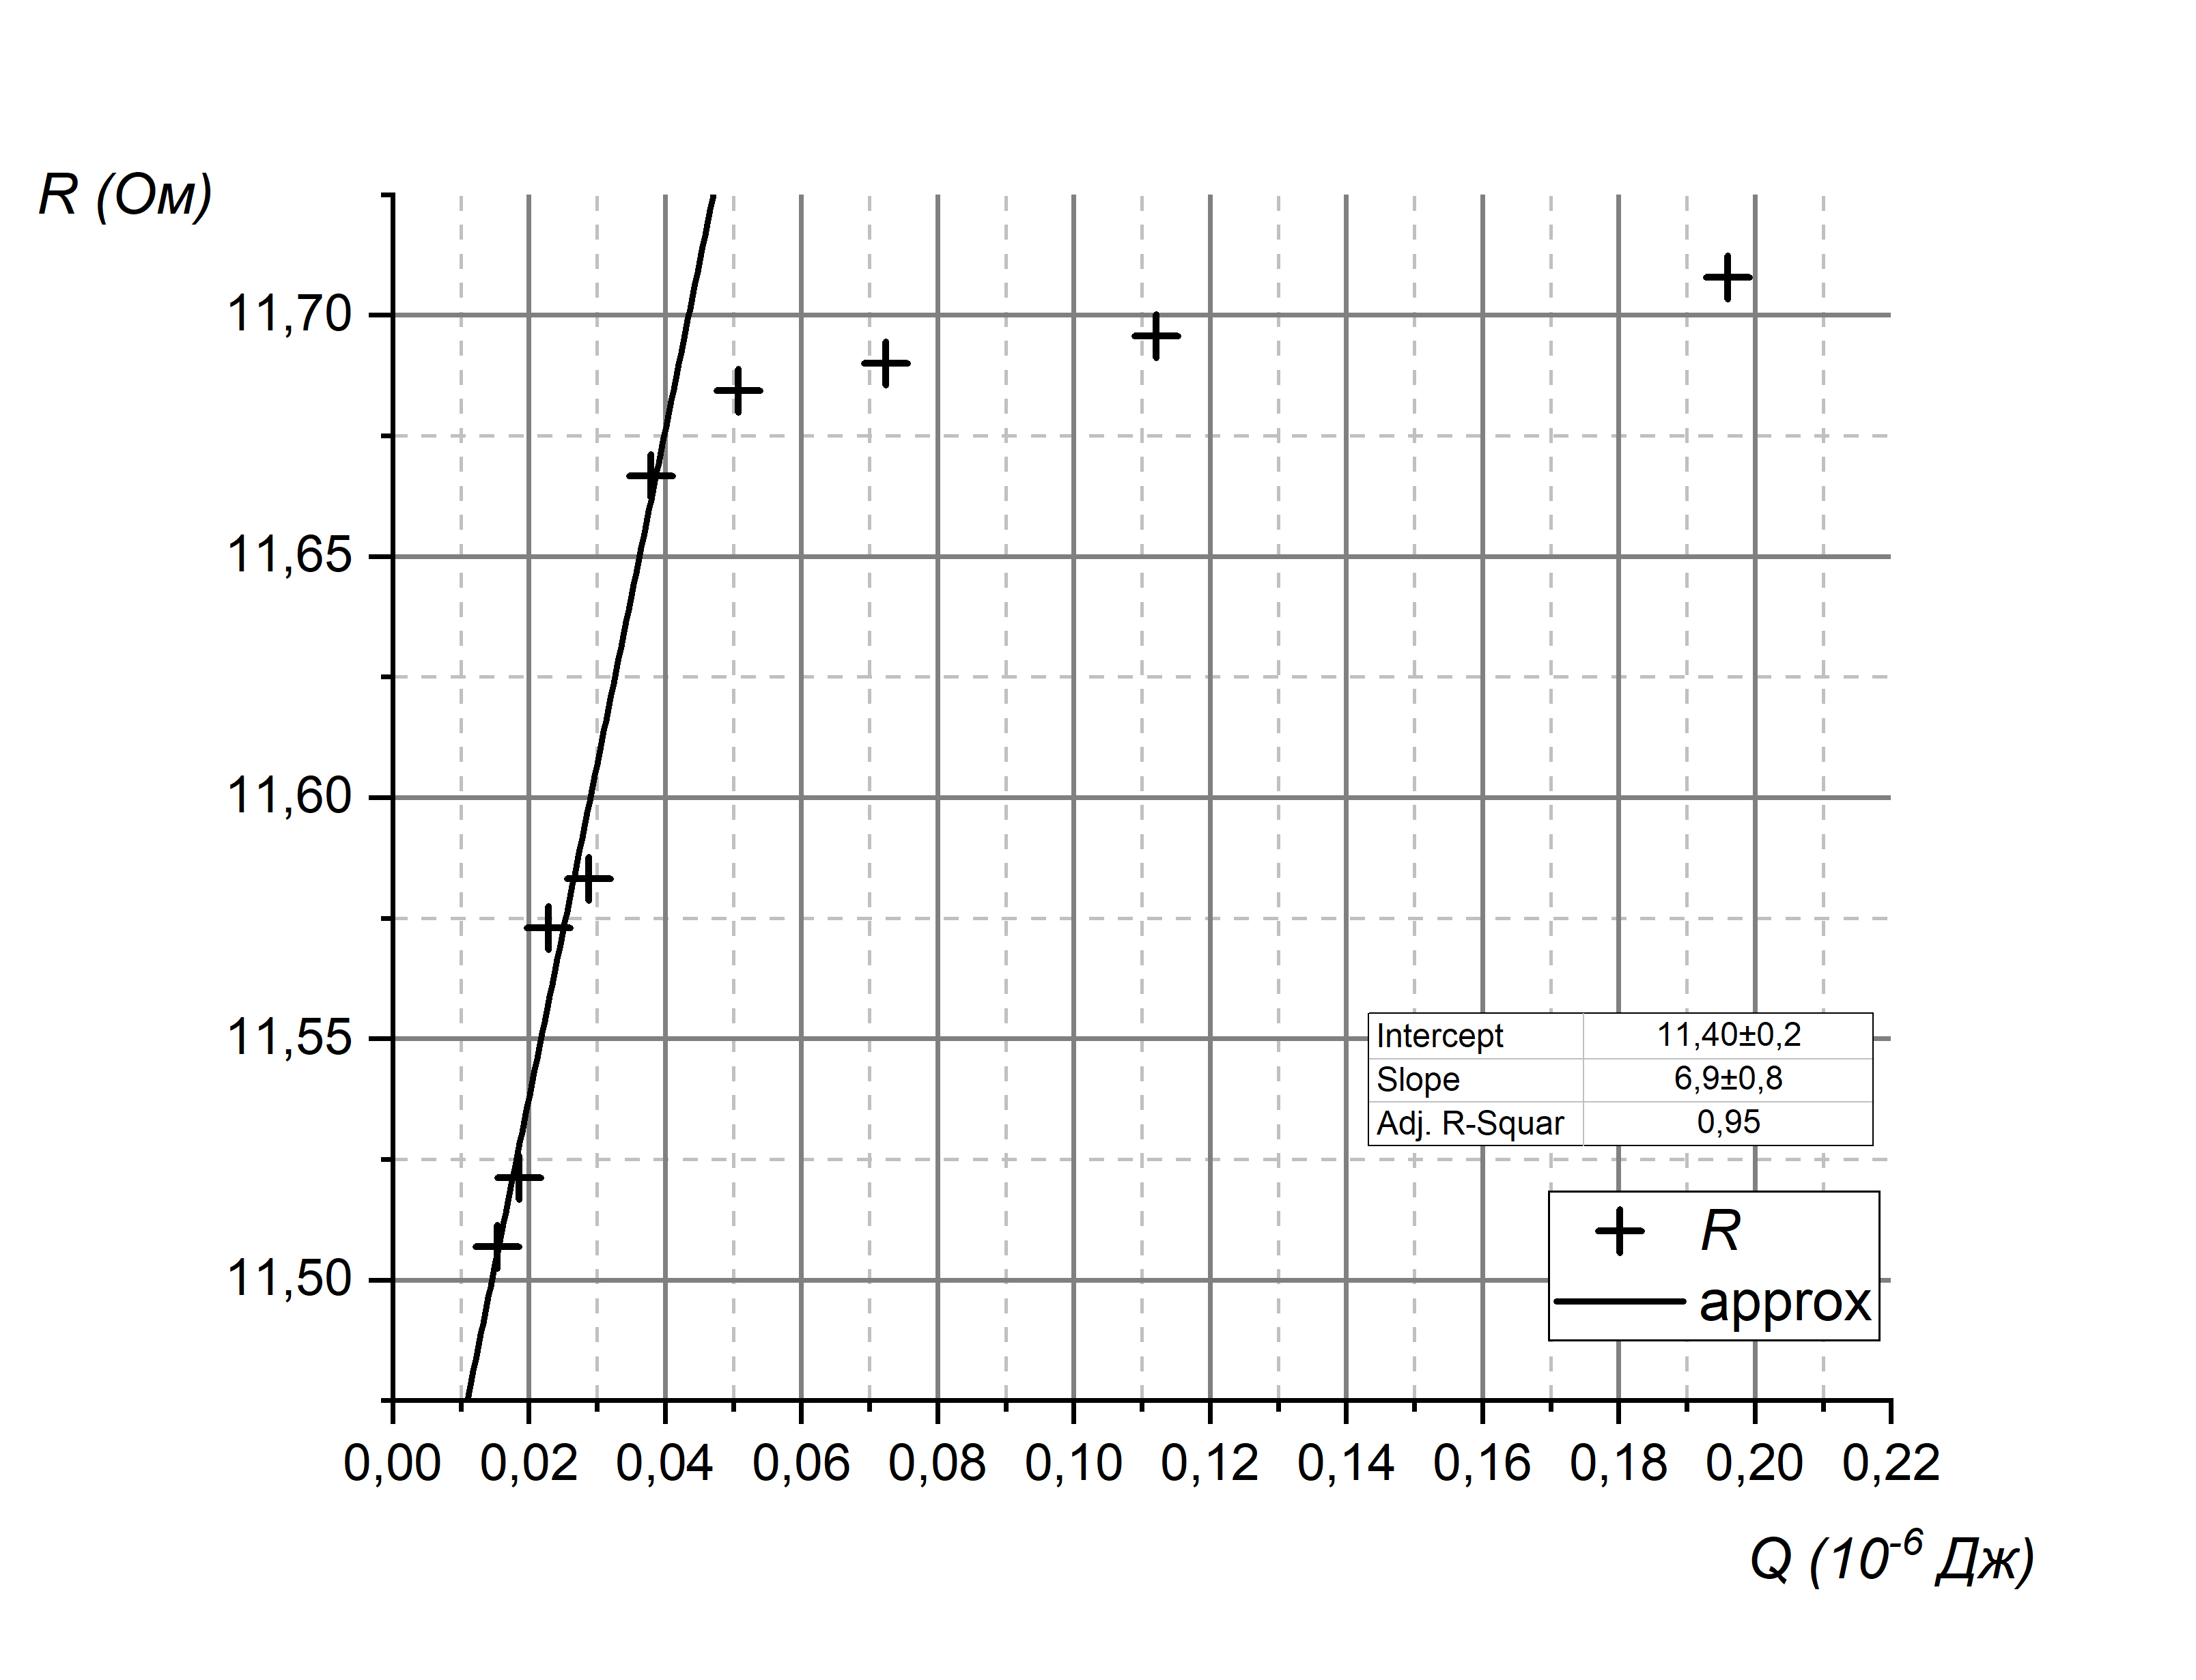
\includegraphics[width = 0.9\textwidth]{2.jpg}}
\caption{График для $T = 35 ^0 C$}
\end{figure}
\FloatBarrier
\FloatBarrier
\begin{figure}[h]
\center{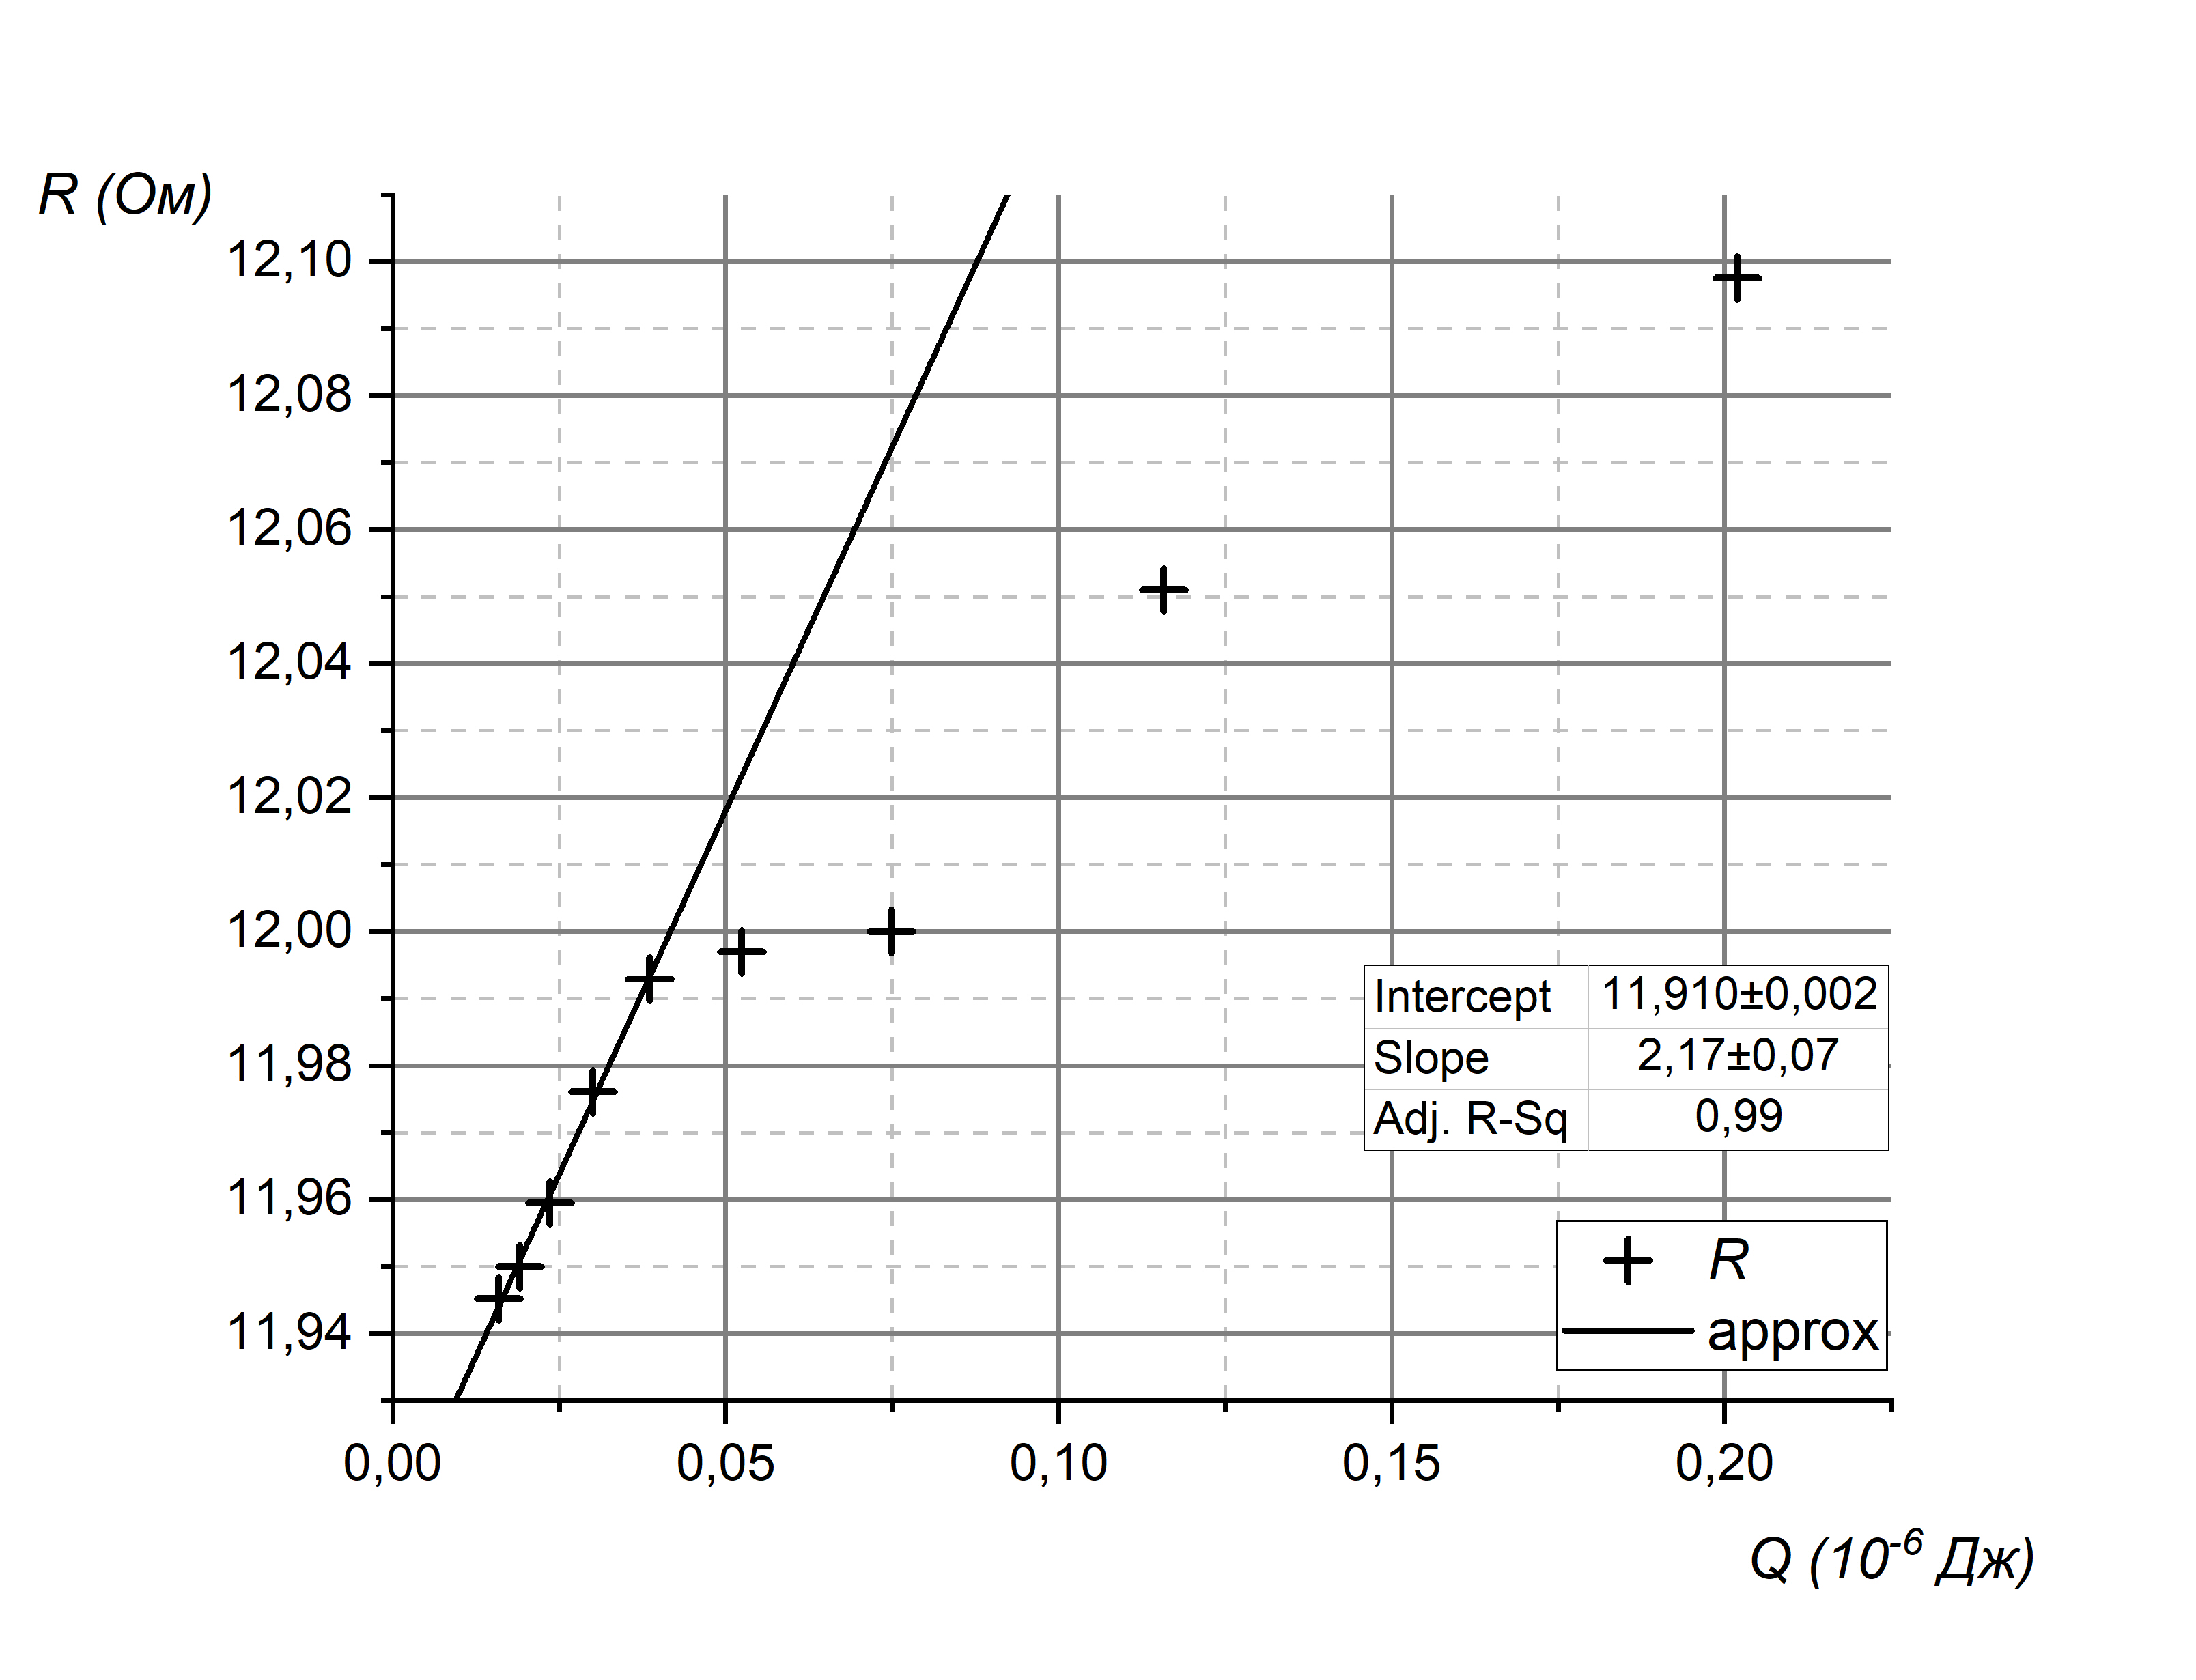
\includegraphics[width = 0.9\textwidth]{3.jpg}}
\caption{График для $T = 45 ^0 C$}
\end{figure}
\FloatBarrier
\FloatBarrier
\begin{figure}[h]
\center{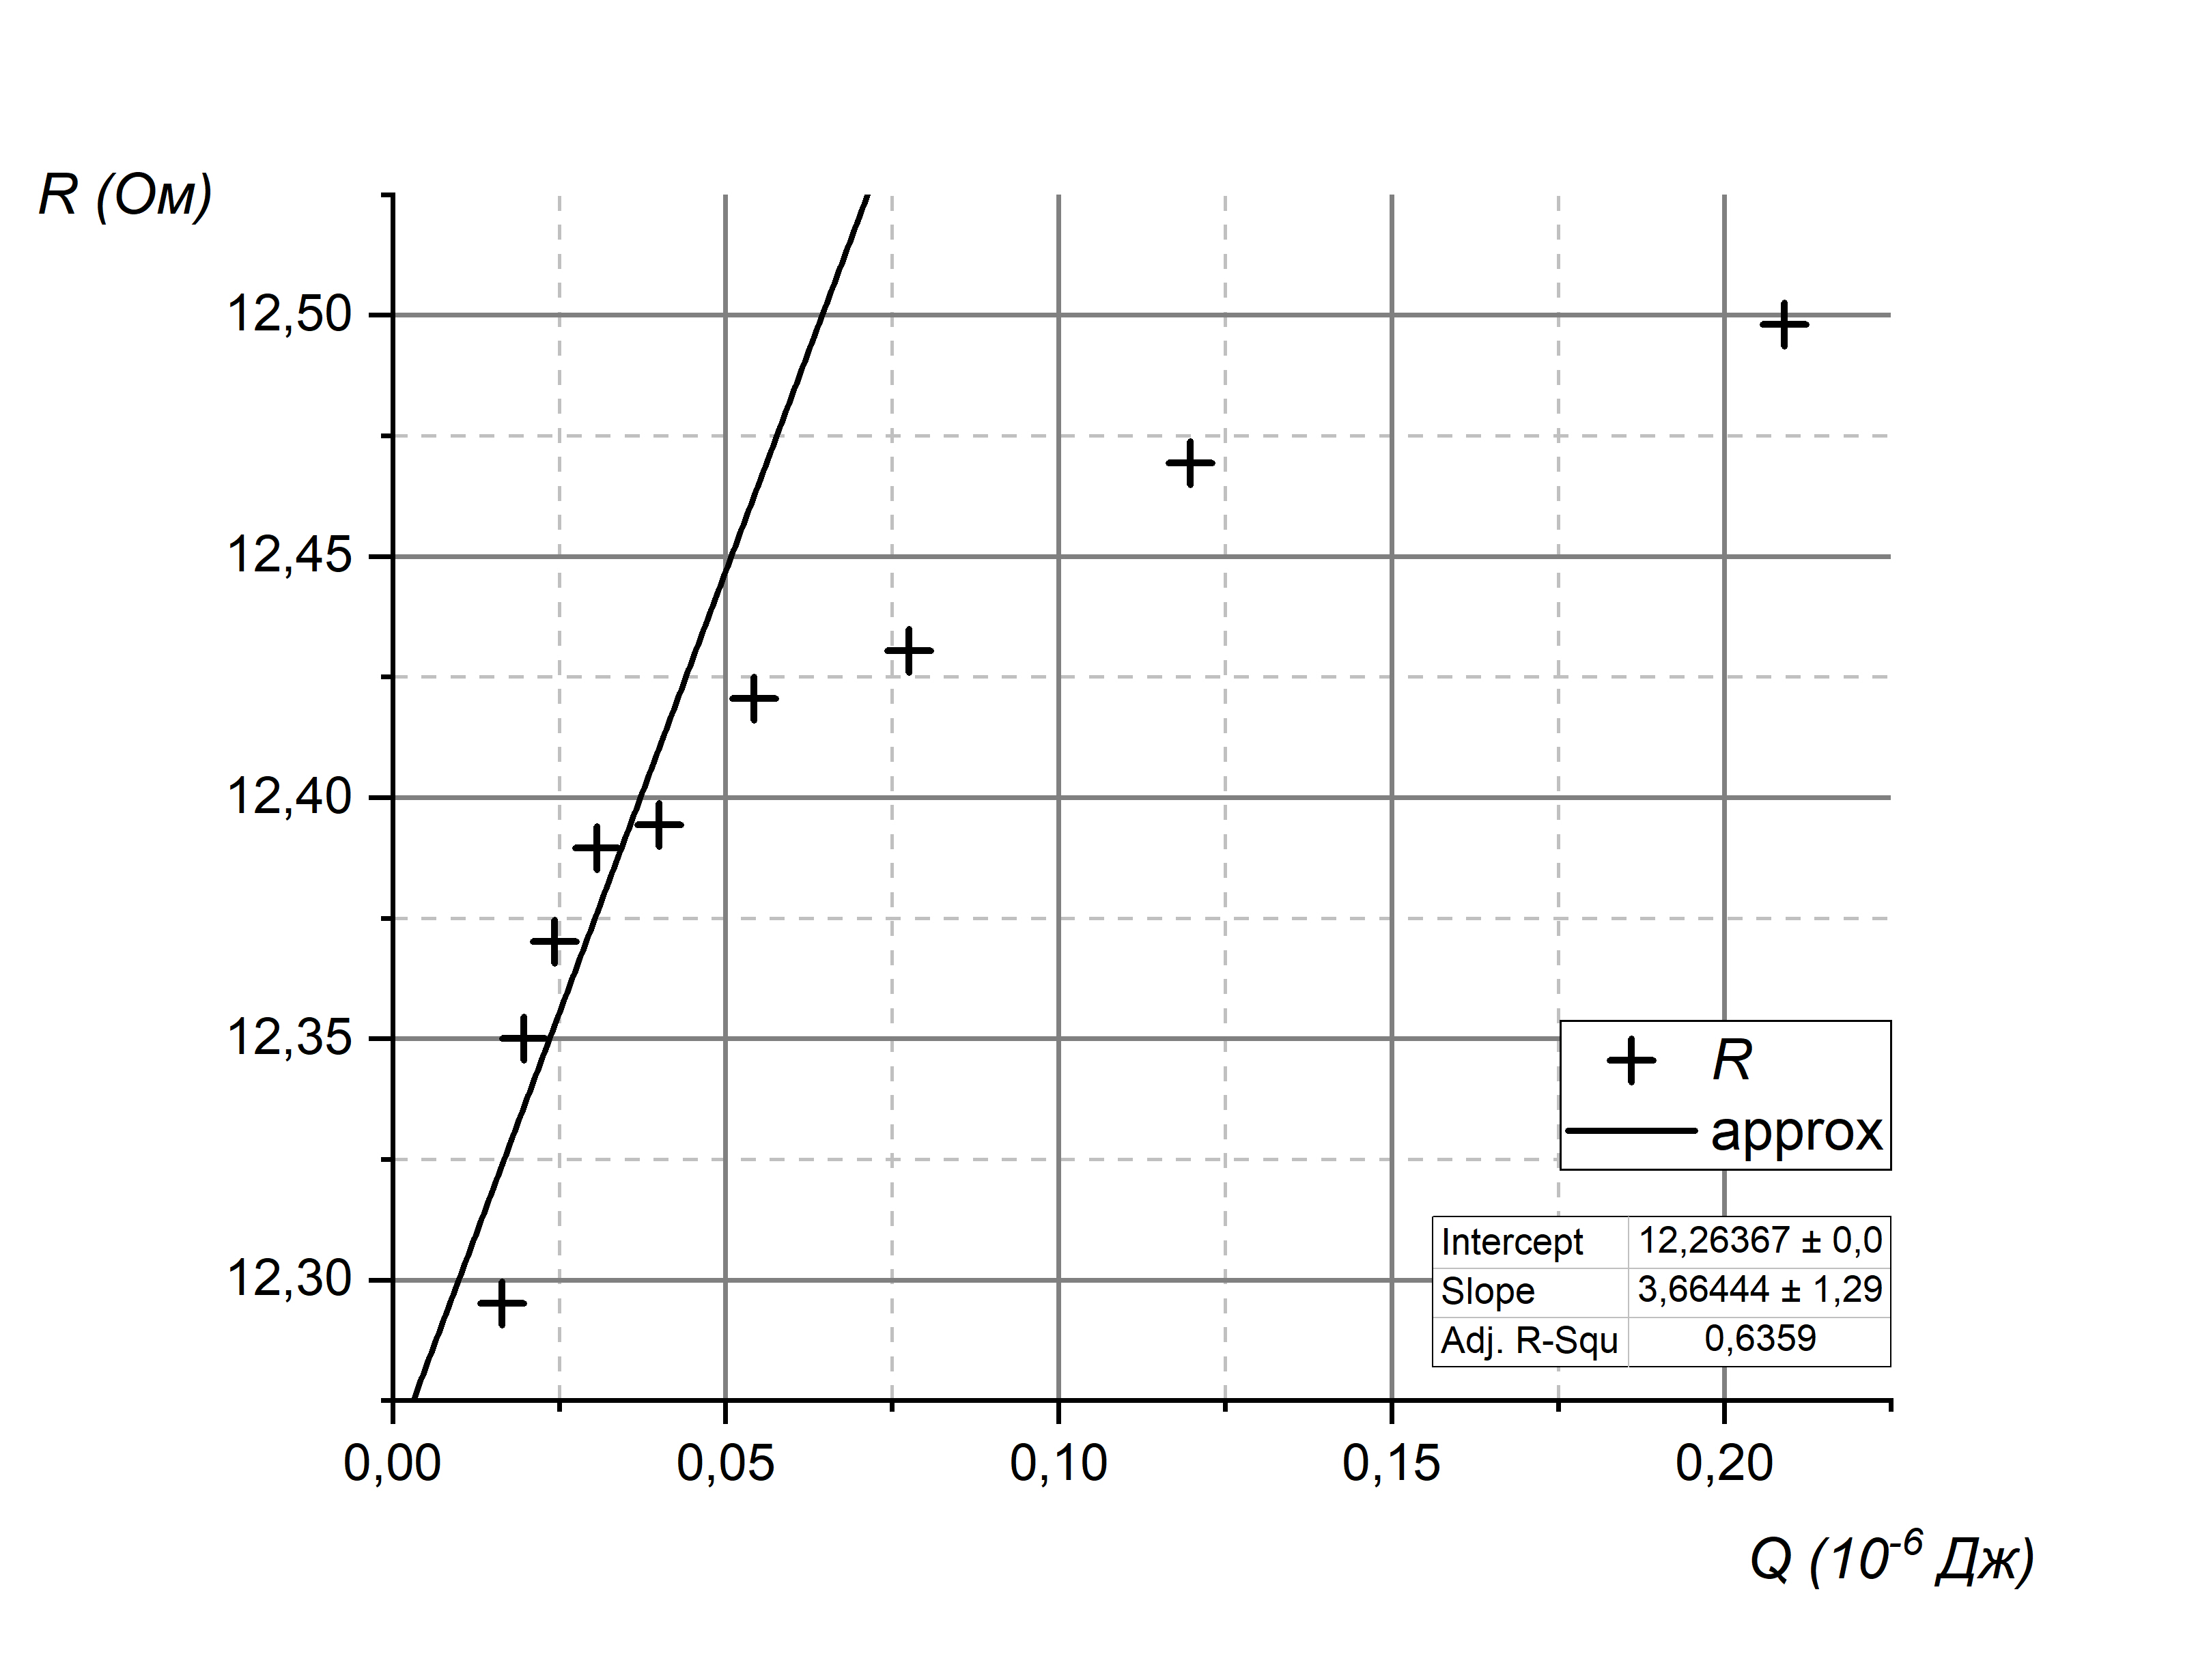
\includegraphics[width = 0.9\textwidth]{4.jpg}}
\caption{График для $T = 55 ^0 C$}
\end{figure}
\FloatBarrier
\FloatBarrier
\begin{figure}[h]
\center{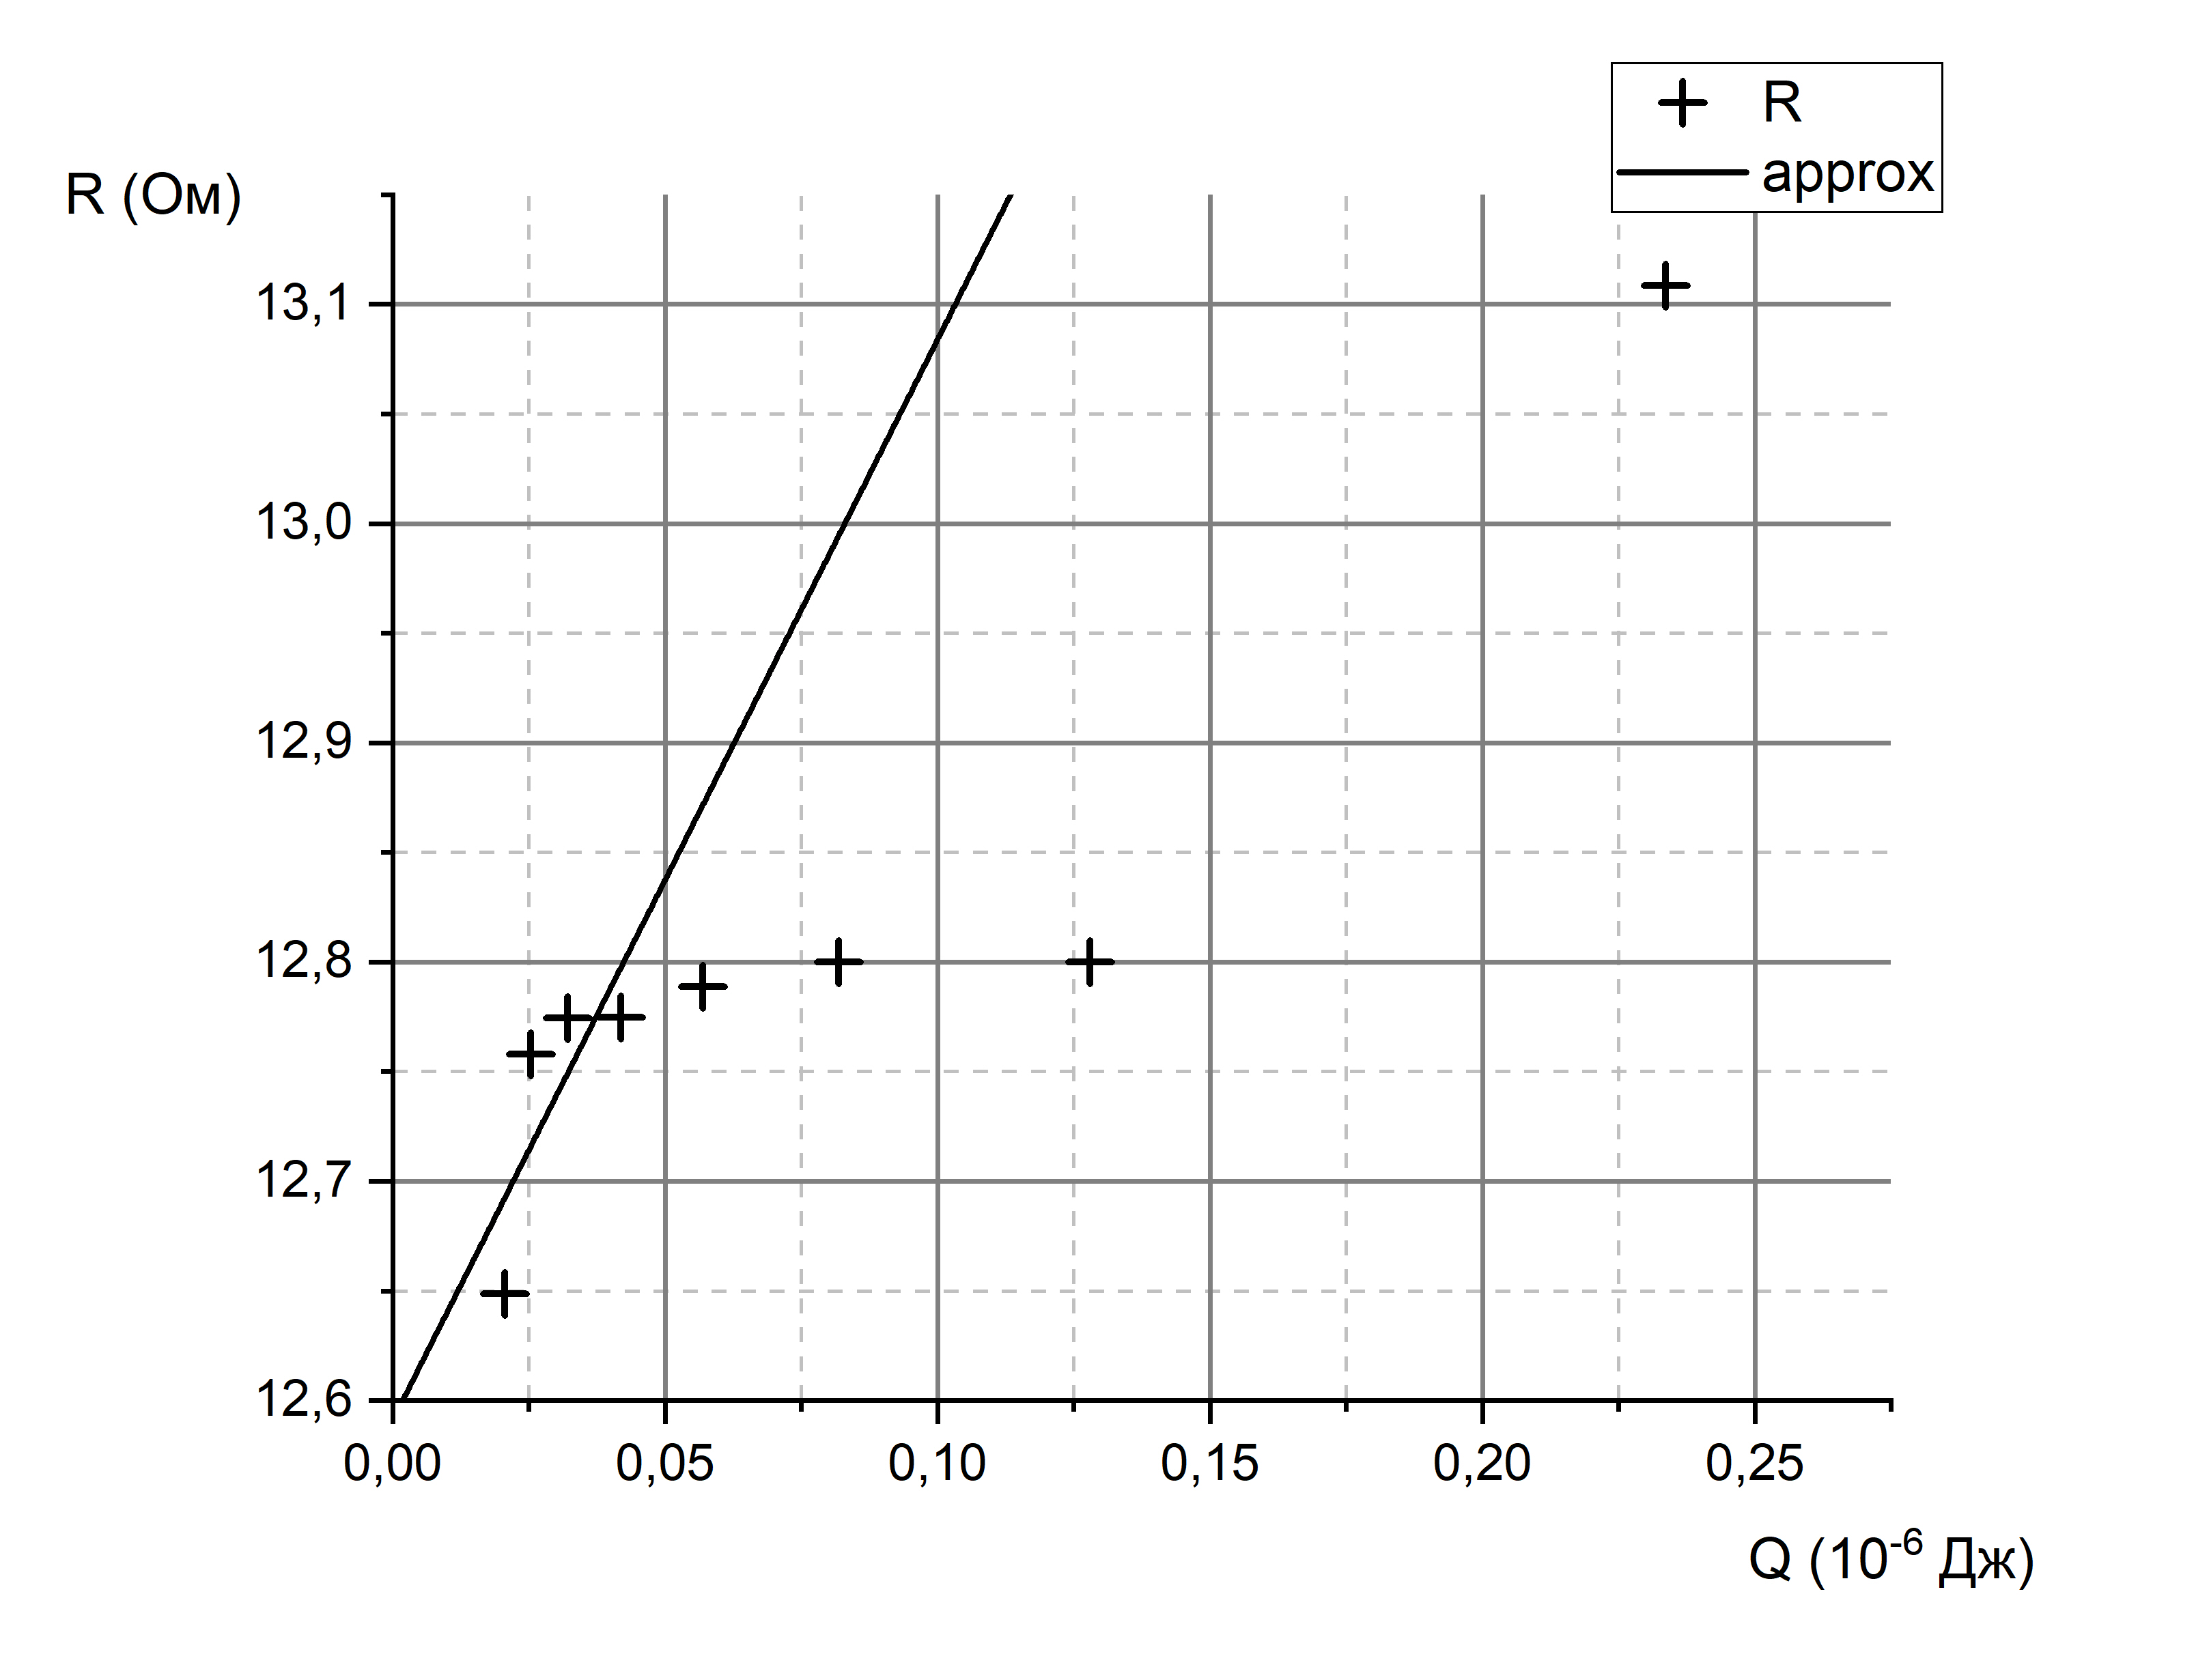
\includegraphics[width = 0.9\textwidth]{5.jpg}}
\caption{График для $T = 65 ^0 C$}
\end{figure}
\FloatBarrier
\FloatBarrier
\begin{figure}[h]
\center{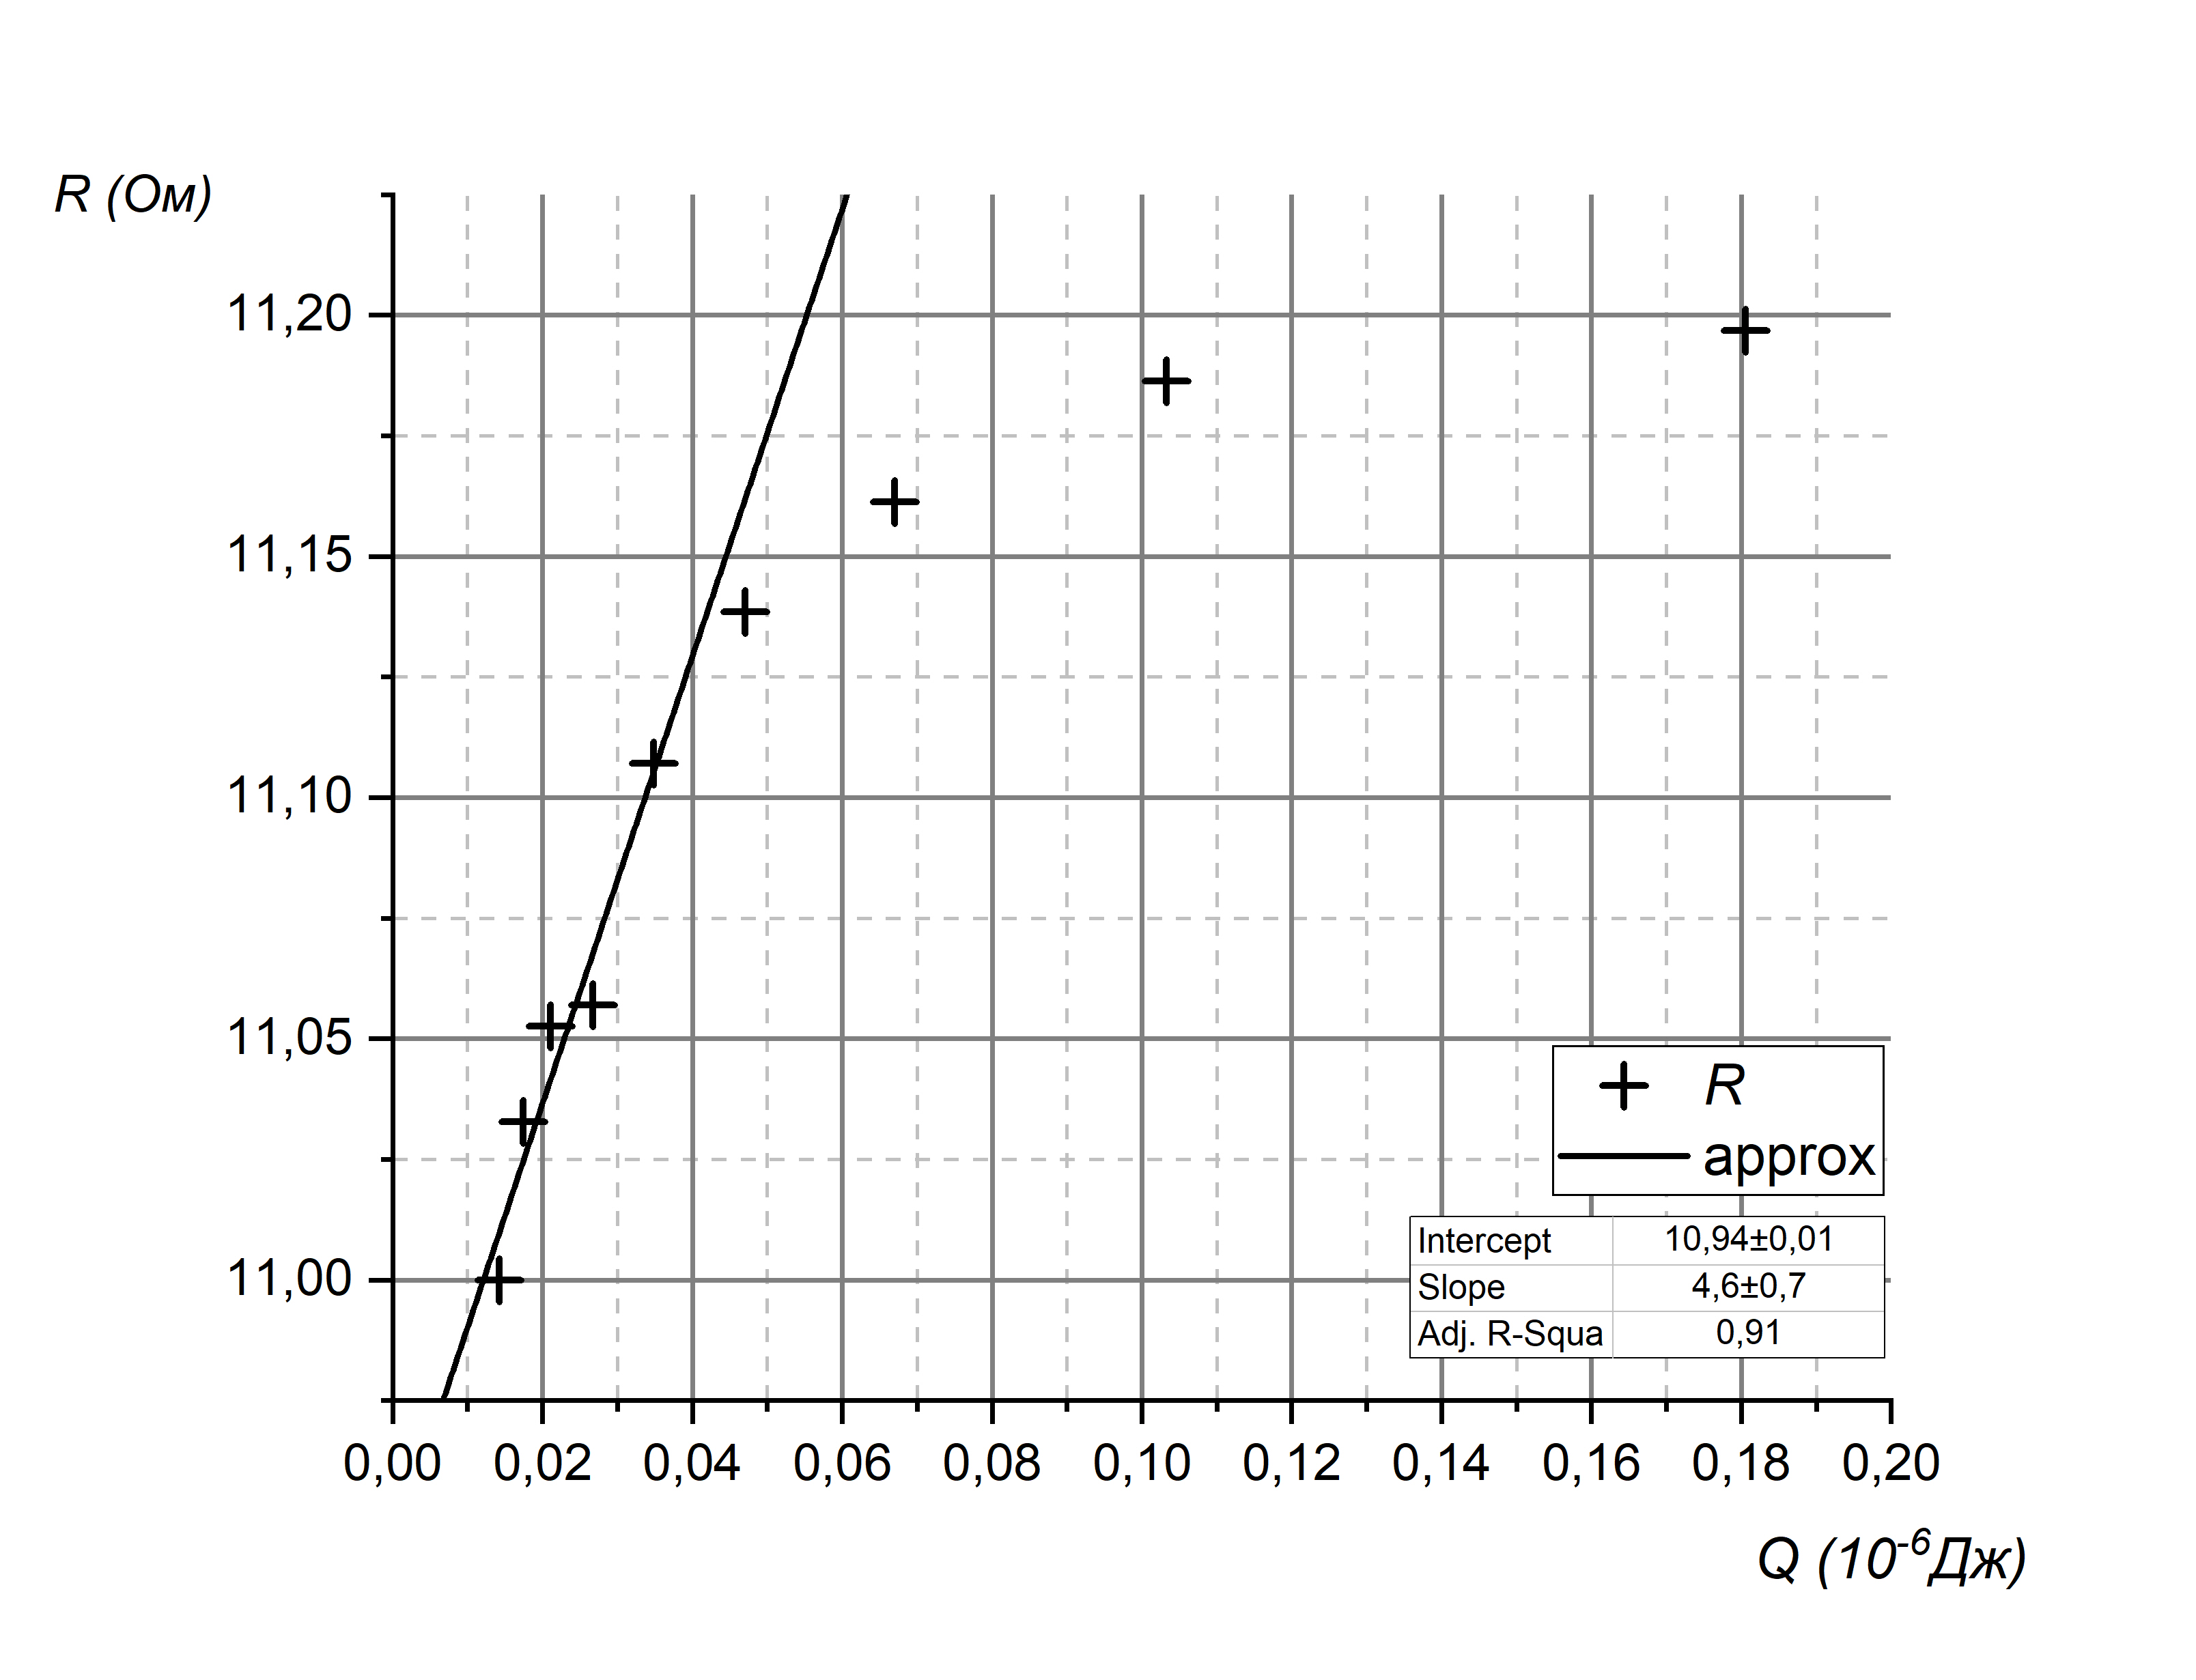
\includegraphics[width = 0.9\textwidth]{6.jpg}}
\caption{График для $T = 70 ^0 C$}
\end{figure}
\FloatBarrier
\item теперь обработаем результаты, запишем все наклоны и $R_0$ из графиков в одну таблицу
\begin{table}[h]
\begin{tabular}{|c|c|c|c|c|}
\hline
$T$, K & $dR/dQ$, Ом/Дж & $\sigma_{dR/dQ}$,  Ом/Дж & $R_0$, Ом & $\sigma_{R_0}$, Ом \\ \hline
298 & 3,4 & 0,8 & 11,07 & 0,03 \\ \hline
308 & 6,9 & 0,8 & 11,4 & 0,2 \\ \hline
318 & 2,17 & 0,07 & 11,910 & 0,002 \\ \hline
328 & 3,7 & 1,3 & 12,27 & 0,01 \\ \hline
338 & 4,6 & 1 & 12,6 & 0,1 \\ \hline
\end{tabular}
\end{table}
\FloatBarrier
\begin{figure}[h]
\center{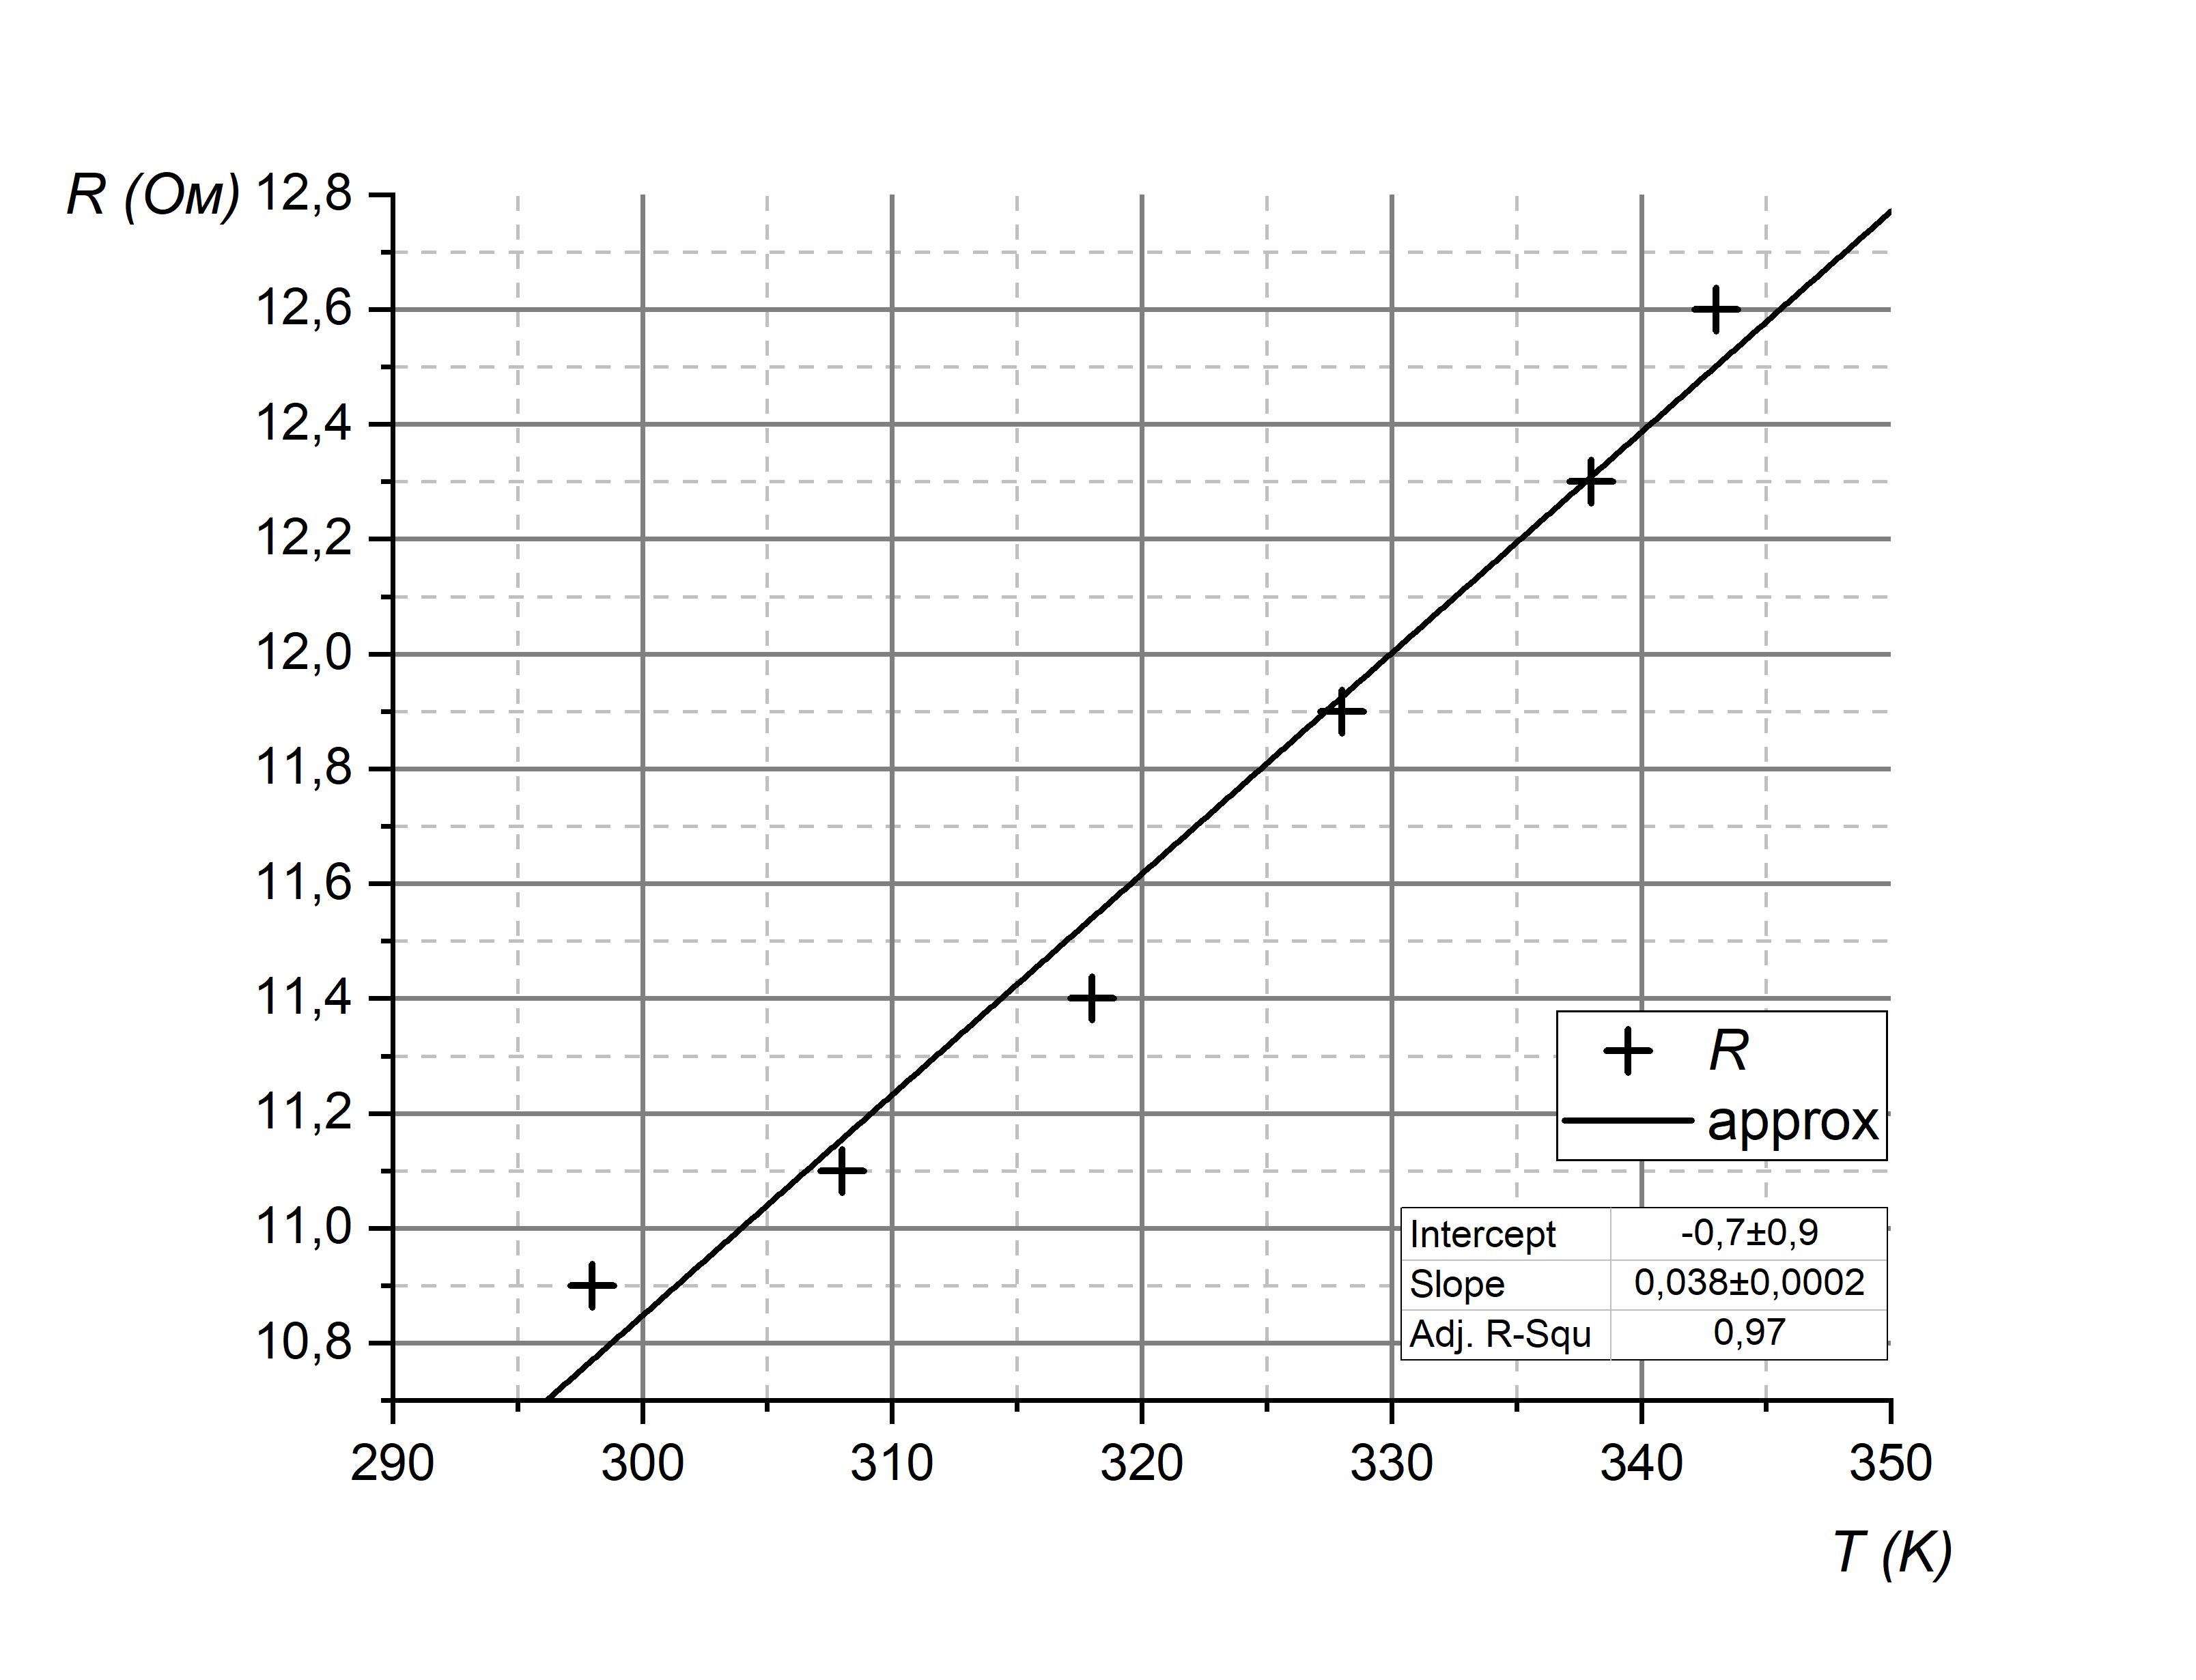
\includegraphics[width = 0.9\textwidth]{9.jpg}}
\caption{График $R(T)$}
\end{figure}
\FloatBarrier
\begin{table}[h]
\begin{tabular}{|c|c|c|c|c|c|c|}
\hline
$T$, K & $dR/dQ$, Ом/Дж & $R_0$, Ом & $\sigma_{R_0}$, Ом & $(dR/dT)/(dR/dQ)$, Дж/К & $k$, Вт/м К & $\sigma_k$, Вт/м К \\ \hline
298 & 3,4 & 11,07 & 0,03 & 0,011 & 0,023 & 0,002 \\ \hline
308 & 6,9 & 11,4 & 0,2 & 0,006 & 0,012 & 0,002 \\ \hline
318 & 2,17 & 11,91 & 0,002 & 0,018 & 0,037 & 0,002 \\ \hline
328 & 3,7 & 12,27 & 0,01 & 0,010 & 0,022 & 0,002 \\ \hline
338 & 4,6 & 12,6 & 0,1 & 0,008 & 0,017 & 0,002 \\ \hline
\end{tabular}
\caption{Таблица $k$}
\end{table}
\end{enumerate}
\end{document}